%\subsection{深度迁移学习 (deep TL)}

\begin{frame}
    \frametitle{迁移学习:深度迁移学习}
    \begin{itemize}
        \item 利用深度神经网络的结构进行迁移学习
            \begin{itemize}
                \item 多层次的特征学习
            \end{itemize}
        \item 代表方法
            \begin{itemize}
                \item Joint CNN [Tzeng, ICCV-15]
                \item SHL-MDNN [Huang, ICASSP-13]
                \item Deep Adaptation Network (DAN) [Long, ICML-15]
                \item Domain Adversarial Training (DANN) [Ganin, ICML-15]
                \item Domain Separation Network (DSN) [Bousmalis, NIPS-16]
                \item Selective Adversarial Network (SAN) [Cao, CVPR-18]
            \end{itemize}
    \end{itemize}
\end{frame}

\begin{frame}
    \frametitle{迁移学习:深度迁移学习}
    \begin{itemize}
        \item 深度学习模型的迁移:定量分析
            \begin{itemize}
                \item unsupervised domain adaption Amazon‑>Webcam over time
            \end{itemize}
    \end{itemize}
    \begin{figure}
        \includegraphics[width=0.9\textwidth]{deep1.png}
    \end{figure}
\end{frame}

\begin{frame}
    \frametitle{迁移学习:深度迁移学习}
    \begin{itemize}
        \item Transferability of Layer‑wise Features \footfullcite{yosinski2014transferable}
    \end{itemize}
    \begin{figure}
        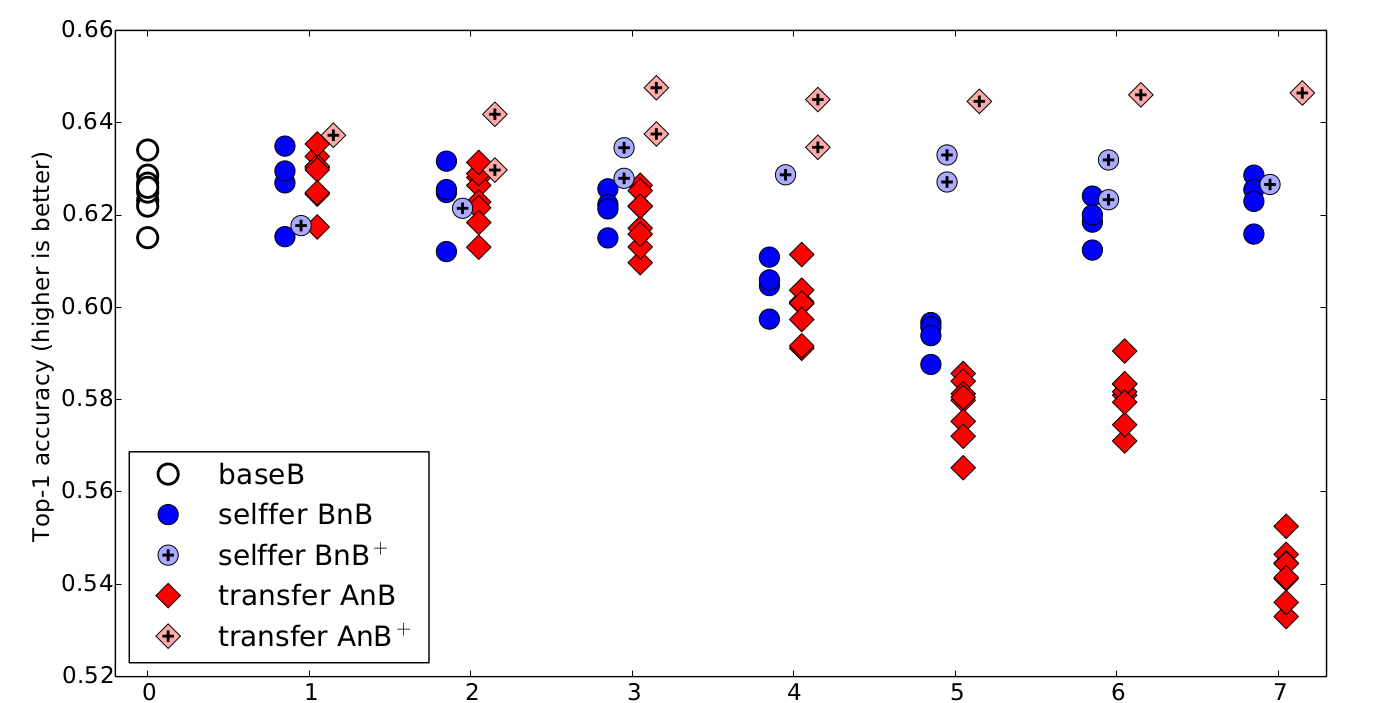
\includegraphics[width=0.8\textwidth]{transferable.png}
    \end{figure}
\end{frame}

\begin{frame}
    \frametitle{迁移学习:深度迁移学习}
    \begin{itemize}
        \item joint CNN [Tzeng, ICCV-15]
            \begin{itemize}
                \item 针对有稀疏标记的目标域数据,用CNN同时优化域之间的距离和迁移学习任务的损失
            \end{itemize}
    \end{itemize}
    \begin{figure}
        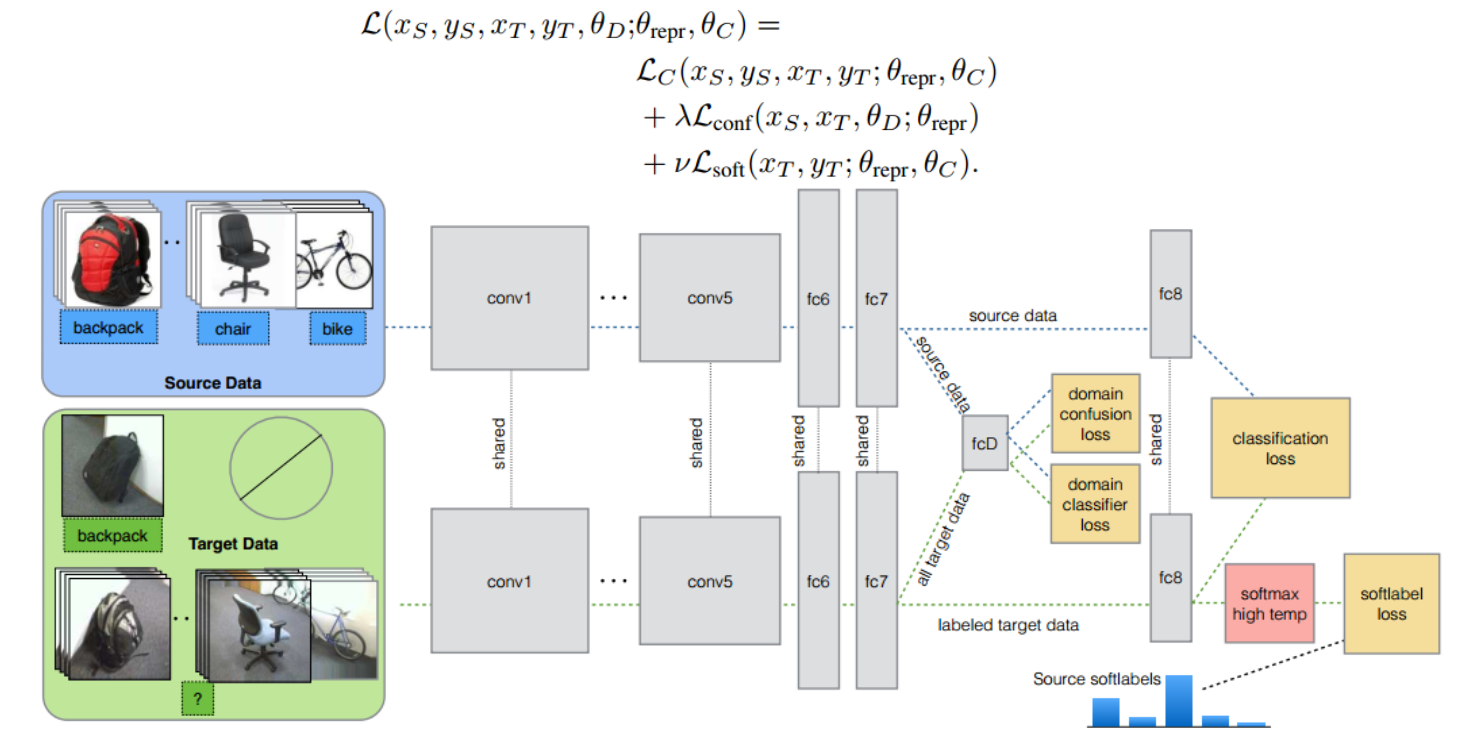
\includegraphics[width=0.9\textwidth]{jcnn.png}
    \end{figure}
\end{frame}

\begin{frame}
    \frametitle{迁移学习:深度迁移学习}
    \begin{itemize}
        \item SHL-MDNN [Huang, ICASSP-13]
            \begin{itemize}
                \item 在不同的学习网络之间共享隐藏层,通过不同的softmax层控制学习任务的不同
            \end{itemize}
    \end{itemize}
    \begin{figure}
        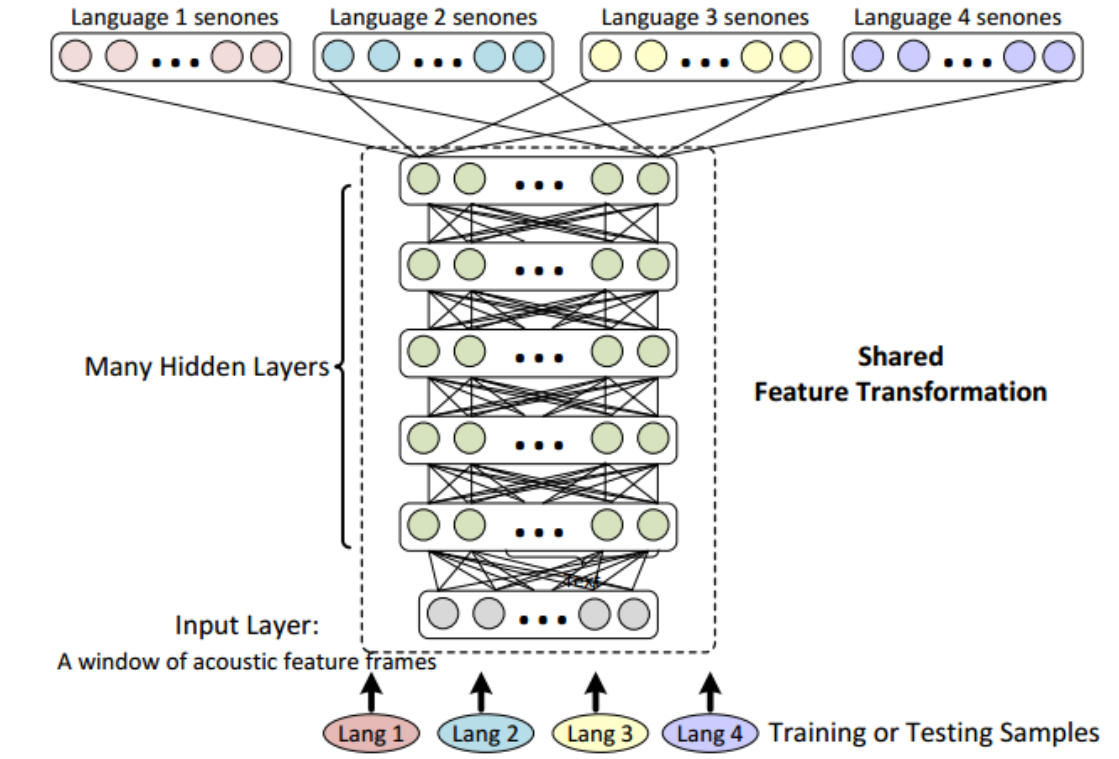
\includegraphics[width=0.7\textwidth]{shl-mdnn.png}
    \end{figure}
\end{frame}

\begin{frame}
    \frametitle{迁移学习:深度迁移学习}
    \begin{itemize}
        \item Deep Adaptation Network (DAN)
    \end{itemize}
    \begin{figure}
        \includegraphics[width=0.8\textwidth]{dan.png}
    \end{figure}
\end{frame}

\begin{frame}
    \frametitle{迁移学习:深度迁移学习}
    \begin{itemize}
        \item Domain Adversarial Training (DANN) [Ganin, ICML-15]
    \end{itemize}
    \begin{figure}
        \includegraphics[width=0.9\textwidth]{dann.png}
    \end{figure}
\end{frame}

\begin{frame}
    \frametitle{迁移学习:深度迁移学习}
    \begin{itemize}
        \item Domain Separation Network (DSN) [Bousmalis, NIPS-16]
    \end{itemize}
    \begin{figure}
        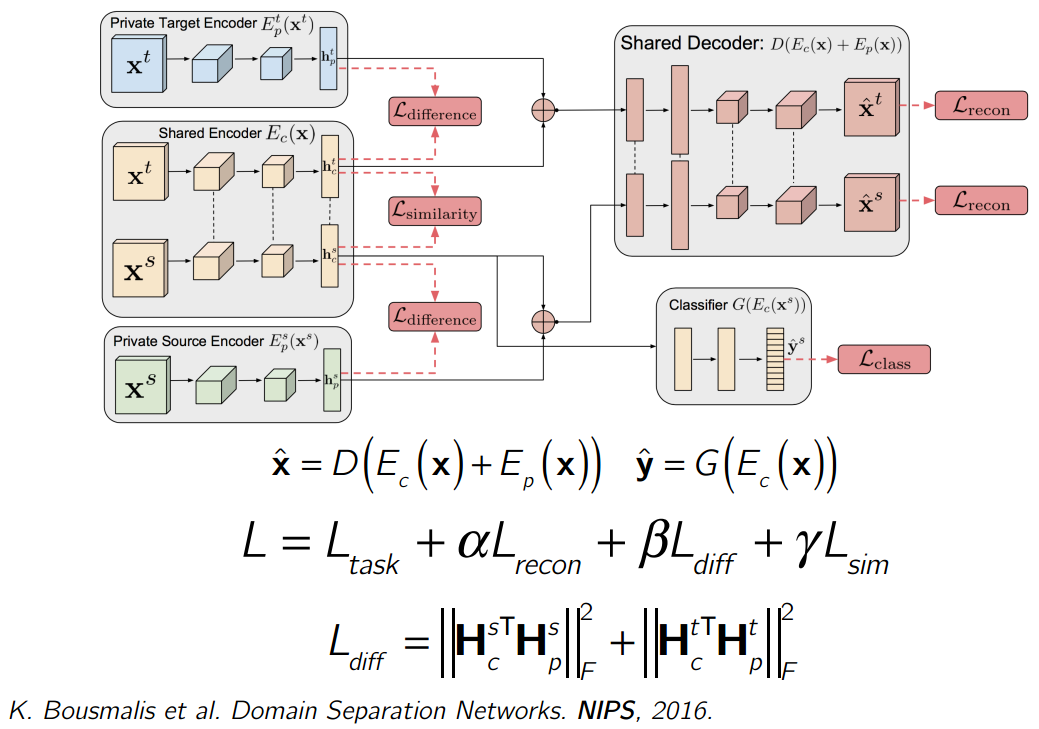
\includegraphics[width=0.8\textwidth]{dsn.png}
    \end{figure}
\end{frame}

\begin{frame}
    \frametitle{迁移学习:深度迁移学习}
    \begin{itemize}
        \item Selective Adversarial Network (SAN) [Cao, CVPR-18]
            \begin{itemize}
                \item Partial Transfer Learning
                \item 源域的标签包含目标域的标签
            \end{itemize}
    \end{itemize}
    \begin{figure}
        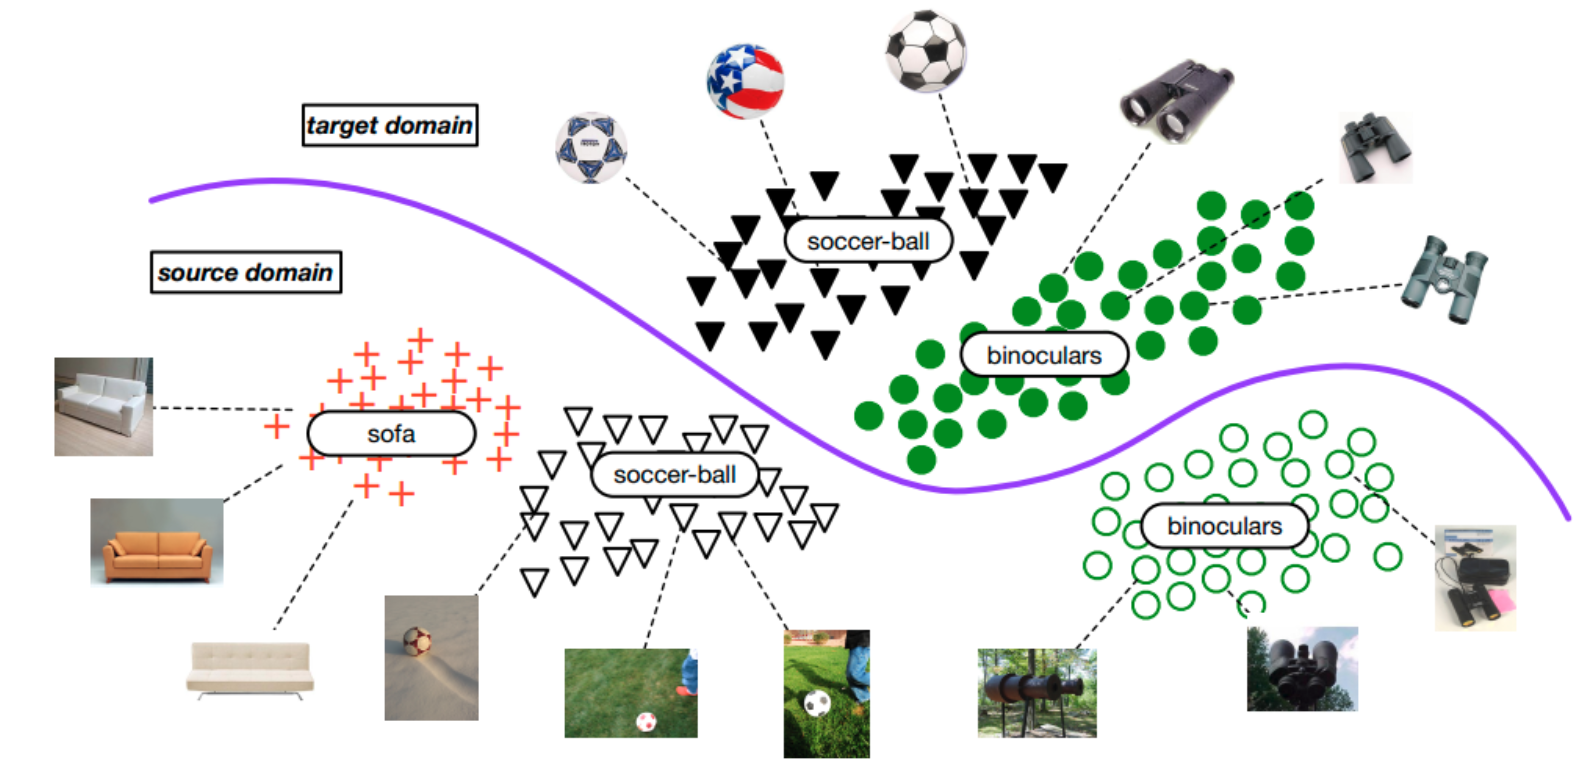
\includegraphics[width=0.8\textwidth]{san1.png}
    \end{figure}
\end{frame}

\begin{frame}
    \frametitle{迁移学习:深度迁移学习}
    \begin{itemize}
        \item Selective Adversarial Network (SAN) [Cao, CVPR-18]
    \end{itemize}
    \begin{figure}
        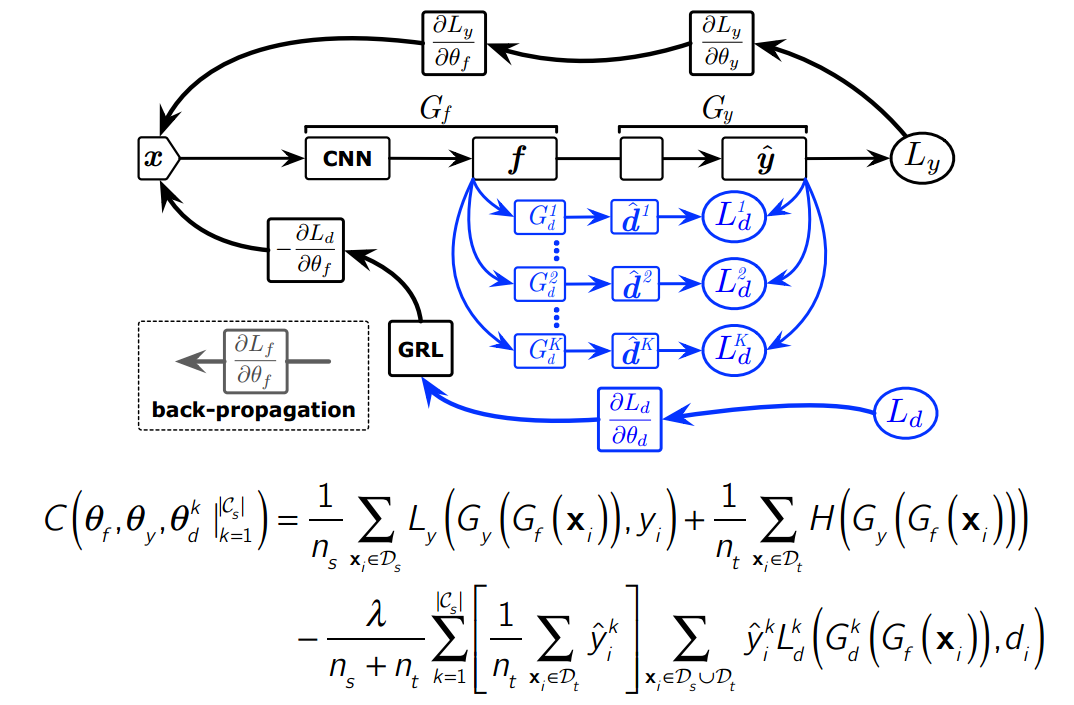
\includegraphics[width=0.8\textwidth]{san2.png}
    \end{figure}
\end{frame}

\begin{frame}
    \frametitle{迁移学习:深度迁移学习}
    \begin{itemize}
        \item 总结
        \begin{itemize}
            \item 迁移学习大增强了模型的泛化能力
            \item 深度学习可以深度表征域中的知识结构
            \item 深度学习+迁移学习还可大有作为
        \end{itemize}
    \end{itemize}
\end{frame}